%###
% \RequirePackage[l2tabu, orthodox]{nag}
\documentclass[a4paper,10pt,twoside]{book}
% \usepackage[width=127mm,height=191mm,includehead,hcentering,vcentering]{geometry}

% \includeonly{_init,basic-concepts,raster}
% \includeonly{__init,k3tree}

% Packages --------------------------------------------------------------------

\usepackage{booktabs,multirow,multicol,array,colortbl,makecell,tabularx} % tablas


\usepackage[width=127mm,height=191mm,includehead,hcentering,vcentering]{geometry}
\usepackage{graphicx,subfigure}				% Include graphics
\usepackage{caption}	% Customize captions
\usepackage[T1]{fontenc} 			% Extended character set
\usepackage{lmodern, microtype}		% Load vector fonts; better text formatting
\usepackage{amsmath,amssymb,amsfonts,amsthm}	% Math support, example environment
\usepackage{fancyhdr} 				% Headers
\usepackage{xspace}	  				% Create macros with appropriate extra space after
\usepackage{lipsum}					% Fill sections
\usepackage{fixltx2e}				% Make math macros robust: \( \) \[ \]



\usepackage[usenames,dvipsnames]{xcolor}	% Colors

\usepackage[chapter]{algorithm}
\usepackage{algorithmicx, algpseudocode}
\usepackage{float}

\usepackage{textcomp, gensymb}	% Common symbols (mu, degree)

%Debug packages
% \usepackage{refcheck}	% Show labels in output pdf. 
						% Note: local refcheck.sty has been modified to solve a bug in handling bibitems 
						% Note 2: since cleveref refcheck is unused




\usepackage{tikz}

\usepackage[breaklinks]{hyperref} % Hyperlinks in refs. Must be loaded at the end (except cleverref)
\usepackage{hypdvips}
% \usepackage[nameinlink]{cleveref}
\usepackage{cleveref}

% \usepackage{theorem}					% Theorems?
% \theoremstyle{plain}
% \newtheorem{definition}{Definition}

% \usepackage{lscape} 					% Set elements to landscape (e.g large figures, tables)
% \usepackage{setspace}					% ??
% \usepackage{rotating}
% \usepackage[tight]{subfigure}
% \usepackage{dcolumn}
% \usepackage[noline,linesnumbered,algochapter]{algorithm2e}
% \providecommand{\DontPrintSemicolon}{\dontprintsemicolon}
% \usepackage{algcompatible}
% \usepackage{sectsty}
%\usepackage[none]{hyphenat}
% \usepackage[tworuled,noline,linesnumbered,algochapter]{algorithm2e}


% FIXME: review in further versions
\hyphenpenalty=5000
\tolerance=1000
\widowpenalty=300
\clubpenalty=300
\emergencystretch=3em

\hfuzz=3em

\usepackage{etoolbox}
\apptocmd{\sloppy}{\hbadness 10000\relax}{}{}	% Avoid ''underfull hbox'' warnings in bibliography


% Separacion entre un parrafo y el siguiente
% \addtolength{\smallskipamount}{-7.60pt}
% \addtolength{\parskip}{.5\baselineskip}%{.5\baselineskip}

% \setlength{\smallskipamount}{-7.60pt}
% \setlength{\parskip}{\smallskipamount}

% Fuente de las subsubsecciones
%\subsubsectionfont{\bf}

\setcounter{tocdepth}{4} \setcounter{secnumdepth}{4}

% Fuentes de los pies de figura
\renewcommand{\captionlabelfont}{\bfseries}
\setlength{\captionmargin}{\parindent}

\renewcommand{\arraystretch}{1.2}	% Adjust vertical margins in tables

%Comandos

\newcounter{example}[chapter]
\def\theexample{\thechapter.\arabic{example}}
\newenvironment{example}{\par\noindent\textbf{Example \refstepcounter{example}\theexample:}}{}

% I need subsubsubsections, but not in the index
\newcommand{\subsubsubsection}[1]{\vspace{2mm}\par\noindent\textbf{#1}}

\renewcommand{\algorithmicrequire}{\textbf{Input:}}
\renewcommand{\algorithmicensure}{\textbf{Output:}}
\newcommand{\Input}{\Require}
\newcommand{\Output}{\Ensure}
\newcommand{\false}{\textbf{false}}
\newcommand{\red}[1]{{\color{red} #1 }}
\newcommand{\blue}[1]{{\color{blue} #1 }}
\newcommand{\cyan}[1]{{\color{cyan} #1 }}
\newcommand{\green}[1]{{\color{green} #1 }}
\newcommand{\todo}[1]{\blue{#1}}
\newcommand{\rewrite}[1]{\cyan{#1}}
\newcommand{\fixme}[1]{{\Large \red{#1}}}

\newcommand*{\irank}[0]{\emph{rank}\xspace}
\newcommand*{\iselect}[0]{\emph{select}\xspace}
\newcommand*{\iaccess}[0]{\emph{access}\xspace}

\DeclareMathOperator\rank{rank}
\DeclareMathOperator\select{select}
\DeclareMathOperator\access{access}

\renewcommand*{\k}[0]{\ensuremath{K}\xspace}
\newcommand*{\kk}[0]{\ensuremath{\k^2}\xspace}
\newcommand*{\kkk}[0]{\ensuremath{\k^3}\xspace}
\newcommand*{\KK}[0]{\ensuremath{\K^2}\xspace}
\newcommand*{\Ktree}[0]{\ensuremath{\k^2}-tree\xspace}
\newcommand*{\ktree}[0]{\ensuremath{\k^2}-tree\xspace}
\newcommand*{\ktrees}[0]{\ensuremath{\k^2}-trees\xspace}
\newcommand*{\Ktrees}[0]{\ensuremath{\k^2}-trees\xspace}
\newcommand*{\koct}[0]{\ensuremath{\k^3}-tree\xspace}
\newcommand*{\Koct}[0]{\ensuremath{\k^3}-tree\xspace}
\newcommand*{\kntree}[0]{\ensuremath{\k^n}-tree\xspace}
\newcommand*{\Kntree}[0]{\ensuremath{\k^n}-tree\xspace}
\newcommand{\kones}[0]{\ensuremath{\k^2}-tree1\xspace}
\newcommand{\koness}[0]{\ensuremath{\k^2}-tree1s\xspace}
\newcommand{\Kones}[0]{\kones}
\newcommand{\kdouble}[0]{\ensuremath{\k^2}-tree1\ensuremath{^{\mathrm{2bits-naive}}}\xspace}
\newcommand{\ksus}[0]{\ensuremath{\k^2}-tree1\ensuremath{^{\mathrm{2bits}}}\xspace}
\newcommand{\kdf}[0]{\ensuremath{\k^2}-tree1\ensuremath{^{\mathrm{df}}}\xspace}
\newcommand{\klevel}[0]{\ensuremath{\k^2}-tree1\ensuremath{^{\mathrm{1-5 bits}}}\xspace}
\newcommand{\Kdouble}[0]{\kdouble}
\newcommand{\Ksus}[0]{\ksus}
\newcommand{\Kdf}[0]{\kdf}
\newcommand{\Klevel}[0]{\klevel}
\newcommand{\btree}[0]{B-tree\xspace}
\newcommand{\btrees}[0]{B-trees\xspace}
\newcommand{\bplus}[0]{B\ensuremath{^+}-tree\xspace}
\newcommand{\bpluss}[0]{B\ensuremath{^+}-trees\xspace}
\newcommand{\dktree}[0]{d\ktree}
\newcommand{\dktrees}[0]{d\ktrees}
\newcommand{\Dktree}[0]{D\ktree}
\newcommand{\Dktrees}[0]{D\dtrees}
\newcommand{\iktree}{I\ktree}
\newcommand{\diktree}{diff-I\ktree}
\newcommand{\mktree}{M\ktree}

\newcommand{\kkind}{M\kones}
\newcommand{\kkacum}{AM\kones}
\newcommand{\ikones}{I\kones}
\newcommand{\koctindex}{\koct}

\newcommand{\diffk}[0]{diffK}
\newcommand{\ediffk}[0]{enh-diffK}
\newcommand{\Diffk}[0]{DiffK}
\newcommand{\Ediffk}[0]{Enh-diffK}

\newcommand{\ktreap}[0]{\ensuremath{\k^2}-treap\xspace}
\newcommand{\ktreaps}[0]{\ensuremath{\k^2}-treaps\xspace}

\newcommand{\ZERO}[0]{0\xspace}
\newcommand{\ZEROS}[0]{0's\xspace}
\newcommand{\ONE}[0]{1\xspace}
\newcommand{\ONES}[0]{1s\xspace}

\newcommand{\dash}[0]{\text{--}}

\newcommand{\kt}[0]{\ensuremath{k}\xspace}

\newcommand{\tdktree}[0]{tt\ktree}


\crefname{algorithm}{Algorithm}{Algorithms}
\crefname{example}{Example}{Examples}
\crefname{part}{Part}{Parts}
\crefname{table}{Table}{Tables}

% \normalfont
% \DeclareFontShape{T1}{lmr}{bx}{sc} { <-> ssub * cmr/bx/sc }{}

\normalfont
\DeclareFontShape{T1}{lmr}{bx}{sc} { <-> ssub * cmr/bx/sc }{}

%%%%%%%%%%%%%%%%%%%%%%%%%%%%%%%%%%%%%%%%%%%%%%%%%%%%%%%%%%%
%%%%%%%%%%%%%%%% Sandbox
% \DeclareSymbolFont{sfoperators}{OT1}{cmss}{m}{n}
% \DeclareSymbolFontAlphabet{\mathsf}{sfoperators}
% 
% \makeatletter
% % \def\operator@font{\mathgroup\symsfoperators}
% \def\select@font{\mathgroup\symsfoperators}
% \makeatother
% 
% \makeatletter
% \def\rank@font{\sf}
% \def\select@font{\bf}
% \makeatother

% \newcommand{\rank}[0]{\ensuremath{\mathrm{rank}}\xspace}
% \newcommand{\select}[0]{\ensuremath{\mathrm{select}}\xspace}
% \newcommand{\irank}[0]{\emph{rank}\xspace}
% \newcommand{\iselect}[0]{\emph{select}\xspace}
% \def\rank{\ensuremath{\mathsf{rank}}}
% \def\select{\ensuremath{\mathsf{select}}}
% \DeclareMathOperator\rank{rank}
% \DeclareMathOperator\select{select}

%%%%%%%%%%%%%% End sandbox
%%%%%%%%%%%%%%%%%%%%%%%%%%%%%%%%%%%%%%%%%%%%%%%%%%%%%


\begin{document}

\pagenumbering{roman}
\pagestyle{fancy}\fancyfoot{}\fancyhead{}
\fancyhead[LO]{\slshape\nouppercase{\rightmark}}
\fancyhead[RE]{\slshape\nouppercase{\leftmark}}
\fancyhead[RO,LE]{\slshape \thepage}

\frontmatter

\begin{titlepage}


\vspace*{0.9cm}

\noindent {\Huge Compressed Data Structures\\ for Trajectory Representation}

\vspace*{1.5cm}

\noindent {\huge Autor: Daniil Galaktionov Hodovaniuk}


\definecolor{rosaudc}{RGB}{198, 0, 126}
\noindent \textcolor{rosaudc}{\rule{\textwidth}{2mm}}

{\large
  \noindent Tesis doctoral UDC / 2019

  \vspace*{1.5cm}

  \noindent Directores: \\Antonio Fari\~na Mart\'inez \\ Nieves Rodr\'iguez Brisaboa
  
  \vspace*{1.0cm}
  
  \noindent Tutor y Director por parte de la empresa: \\Eduardo Rodr\'iguez L\'opez

  \vspace*{1.5cm}

 % \noindent Programa Oficial de Doutoramento en Computaci\'on
}

\begin{center}
  \vspace*{1.9cm}
  
\includegraphics[scale=0.20]{figures/_init/udc-color}
\end{center}


\end{titlepage}

\thispagestyle{empty}

%\begin{titlepage}
%\begin{center}
%
%%\vspace*{0.9cm}
%
%
\includegraphics[scale=0.30]{figures/_init/udc-color}
%
%\vspace*{1.2cm}
%
%%{\large \sc Departamento de Computaci\'on, Universidade da Coru\~na} \\[5mm]
%%{\large \scshape Departamento de Computaci\'on} \\[5mm]
%%{\large } \\[2mm]
%%{\Large \scshape Proyecto fin de carrera \\ de Ingenier�a Inform�tica} \\
%
%\vspace*{2.5cm}
%
%{\LARGE \textsc{\textbf Compact data structures for large and complex datasets}}
%
%\end{center}
%
%\vspace*{2.8cm}
%
%\begin{center}
%%\large \bf
%\large
%{\Large \textsc{\textbf{Tesis Doctoral}}} \\[1.8cm]
%{{Doctorando:}  %\\[2mm]
%Fernando Silva Coira}\\[4mm]
%{{Directores:} %\\[2mm]
%Susana Ladra Gonz\'alez, Jos\'e Ram\'on Param\'a Gab\'ia}\\[1.2cm]
%{A Coru\~na, Julio de 2017}
%\end{center}
%
%\end{titlepage}
%
%\thispagestyle{empty}

\begin{titlepage}


\vspace*{0.9cm}

\noindent {\Huge Trust me I'm a Doctor}

\vspace*{1.5cm}

\noindent {\huge Autor: Daniil Galaktionov Hodovaniuk}


\definecolor{rosaudc}{RGB}{198, 0, 126}
\noindent \textcolor{rosaudc}{\rule{\textwidth}{2mm}}

{\large
  \noindent Tesis doctoral UDC / 2019

  \vspace*{1.5cm}

  \noindent Directores: \\Antonio Fari\~na Mart\'inez \\ Nieves Rodr\'iguez Brisaboa
  
  \vspace*{1.5cm}

  \noindent Programa Oficial de Doutoramento en Computaci\'on
}

\begin{center}
  \vspace*{1.9cm}
  
\includegraphics[scale=0.20]{figures/_init/udc-color}
\end{center}


\end{titlepage}

\thispagestyle{empty}

%\begin{titlepage}
%\begin{center}
%
%%\vspace*{0.9cm}
%
%
\includegraphics[scale=0.30]{figures/_init/udc-color}
%
%\vspace*{1.2cm}
%
%%{\large \sc Departamento de Computaci\'on, Universidade da Coru\~na} \\[5mm]
%%{\large \scshape Departamento de Computaci\'on} \\[5mm]
%%{\large } \\[2mm]
%%{\Large \scshape Proyecto fin de carrera \\ de Ingenier�a Inform�tica} \\
%
%\vspace*{2.5cm}
%
%{\LARGE \textsc{\textbf Compact data structures for large and complex datasets}}
%
%\end{center}
%
%\vspace*{2.8cm}
%
%\begin{center}
%%\large \bf
%\large
%{\Large \textsc{\textbf{Tesis Doctoral}}} \\[1.8cm]
%{{Doctorando:}  %\\[2mm]
%Fernando Silva Coira}\\[4mm]
%{{Directores:} %\\[2mm]
%Susana Ladra Gonz\'alez, Jos\'e Ram\'on Param\'a Gab\'ia}\\[1.2cm]
%{A Coru\~na, Julio de 2017}
%\end{center}
%
%\end{titlepage}
%
%\thispagestyle{empty}

\pagebreak \mbox{} \pagebreak
\thispagestyle{empty}

\begin{flushleft}

{\bfseries PhD thesis supervised by} \\[1pt]
{\itshape \bfseries Tesis doctoral dirigida por} \\[4mm]

{\bfseries Antonio Fari\~na Mart\'inez} \\[2pt]
Departamento de Computaci\'on \\[1pt]
Facultad de Inform\'atica \\[1pt]
Universidade da Coru\~na \\[1pt]
15071 A Coru\~na (Espa\~na) \\[1pt]
Tel: +34 981 167000 ext. 1352 \\[1pt]
Fax: +34 981 167160 \\[1pt]
\verb=antonio.farina@udc.es= \\[4mm]

{\bfseries Nieves Rodr\'iguez Brisaboa} \\[2pt]
Departamento de Computaci\'on \\[1pt]
Facultad de Inform\'atica \\[1pt]
Universidade da Coru\~na \\[1pt]
15071 A Coru\~na (Espa\~na) \\[1pt]
Tel: +34 981 167000 ext. 1243 \\[1pt]
Fax: +34 981 167160 \\[1pt]
\verb=brisaboa@udc.es= \\[8mm]

{\itshape \bfseries Tutor y director responsable por parte de la empresa} \\[4mm]

{\bfseries Eduardo Rodr\'iguez L\'opez} \\[2pt]
%Tutor y Director responsable por parte de la empresa \\[1pt]
Enxenio S.L. \\[1pt]
Calle Jos\'e Luis Bugallal Marchesi \\[1pt]
\textnumero~20 1 Izq., 15008 A Coru\~na (Espa\~na) \\[1pt]
Tel: +34 981 913 768 \\[1pt]
\verb=edu@enxenio.es=

\end{flushleft}

Antonio Fari\~na, Nieves Rodr\'iguez Brisaboa y Eduardo Rodr\'iguez, como directores, acreditamos que esta tesis cumple los requisitos para optar a los t\'itulo de doctor industrial e internacional, y autorizamos su dep\'osito y defensa por parte de Daniil Galaktionov Hodovaniuk cuya firma tambi\'en se incluye.




\thispagestyle{plain}
\pagebreak \mbox{} \pagebreak

\vspace*{\stretch{1}}
\begin{flushright} \large \itshape

In the memory of my grandmother.

\end{flushright}
\vspace*{\stretch{1}}

\thispagestyle{empty}

\thispagestyle{plain}
\chapter*{Acknowledgements}
Extended acknowledgements.\\

\vspace*{\fill}
This thesis has received funding from ...

\chapter*{Agradecimientos}
Dedicatoria larga.\\

\vspace*{\fill}
Esta tesis ha recibido fondos ...
\thispagestyle{plain}

\chapter*{Abstract}

The proliferation of GPS devices in smartphones, vehicles and sport wearables on the one hand, and geolocation mechanisms (such as smart cards in public transportation) on the other hand, have led to an unprecedented ability to gather and store trajectories that originate from people's movements during their daily schedules. However, no standard data models exist to represent these trajectories and, in addition, neither traditional databases nor new \textit{NoSQL} databases are adequate for the representation and exploitation of the complex spatio-temporal data that make up such trajectories. This general outlook is even more complex once we consider that whenever we are storing information related to the context of public transportation passengers, customers inside a mall, or simply vehicles moving in a city we must deal with a true Big Data scenario in which guaranteeing an efficient response can be very challenging.

Consequently, in this thesis we address the design of compact data structures for the representation of the followed trajectories, both in the context of vehicles and/or people moving in urban or periurban spaces, as in the context of itineraries of commuters in public transportation. Apart from designing these compact data structures that allow us to represent the Big Data scenario usually seen in this application domain, we have also designed the algorithms that allow the efficient exploitation of the underlying information.

We have implemented algorithms that not only to solve the classic spatio-temporal queries, such as obtaining the position of a moving object at a time instant, reconstructing the trajectory of an object, or even spatio-temporal window queries (which objects are inside a spatial range either within a time window or at a time instant), but also solve more specialized queries for the analysis of the trajectories that travelers make. For instance, we have designed algorithms to query the number of travelers that start (or finish) their trip in a certain place within a given time interval, or the number of travelers that switch from one line from the public transportation network to another one using a particular stop, or even the number of travelers that had started their trip in a certain place (which can be either a stop or a whole neighborhood) and finished it in another place.

Both the designed structures and the querying algorithms, which are available at \url{https://github.com/dgalaktionov/compact-trip-representation}, have been experimentally evaluated. With these structures we were able to represent, in a compact space of 100 MiB, a collection of approximately a million and a half of taxi trajectories, or alternatively ten million trajectories consisting of itineraries over public transportation networks (the latter being more compressible). In both cases, we can solve most of the considered exploitation queries in the order of microseconds, with algorithms that scale logarithmically with respect to the increase in the number of stored trajectories.

Finally, considering that this work is considered an industrial thesis, and that this requires showing that the research performed is of clearly applied nature, we have developed a web application with Geograhic Information Systems technology, which integrates with our compressed structures and algorithms instead of relying on common spatial databases. This application, which provides a simple and intuitive user interface that represents the map of a transportation network, enabled an end user to run the aforementioned querying algorithms over a large collection of historic trajectories. Likewise, this interface presents the query results in a graphical and intuitive way.

\chapter*{Resumen}

La proliferaci\'on de por un lado de dispositivos GPS en smartphones, veh\'iculos o pulseras de deporte,  y por otro, de otros mecanismos de geolocalizaci\'on (como las tarjetas de pago de trasporte p\'ublico), han dado lugar a una capacidad in\'edita de obtener y almacenar las trayectorias que generan las personas al moverse durante sus quehaceres diarios. Sin embargo, no existen modelos de datos est\'andar para representar dichas trayectorias, adem\'as de que ni las bases de datos tradicionales, ni las nuevas bases de datos \textit{NoSQL} se adec\'uan bien a la representaci\'on y explotaci\'on de esos datos complejos de naturaleza espacio-temporal que son las trayectorias.  Para hacer m\'as complejo a\'un el panorama, se constata adem\'as que cuando se quieren almacenar trayectorias de viajeros de transporte p\'ublico, o de clientes en centros comerciales, o simplemente de personas o veh\'iculos movi\'endose por una ciudad hay que enfrentarse a un verdadero escenario Big Data en el que la eficiencia en la respuesta a las consultas se hace muy dif\'icil.

Por todo ello, en esta tesis se aborda el dise\~no de estructuras de datos compactas para la representaci\'on de las trayectorias seguidas, por un lado, por veh\'iculos y/o personas que se mueven por las calles de un entorno urbano o periurbano acotado, y por otro los itinerarios de viajeros de transporte p\'ublico. Adem\'as de dise\~nar esas estructuras de datos compactas, que permiten representar ese escenario Big Data habitual en estos dominios de aplicaci\'on, se han dise\~nado los algoritmos que permiten la explotaci\'on eficiente de dichos datos.

Hemos implementado algoritmos que, adem\'as de resolver las consultas espacio-temporales cl\'asicas, tanto las de posici\'on de un objeto en un tiempo, o trayectoria de un objeto durante un intervalo temporal, como las consultas de rango espacio-temporal (qu\'e objetos est\'an en una ventana del espacio en un instante o intervalo temporal) resuelven tambi\'en consultas m\'as especializadas para el an\'alisis de trayectorias de viajeros. Por ejemplo, hemos dise\~nado algoritmos para  consultar el n\'umero de viajeros que inician (o terminan)  su viaje en un lugar dado dentro de un cierto intervalo temporal, o el n\'umero de viajeros que conmutan de una l\'inea a otra de la red de transporte p\'ublico en una parada concreta, o incluso el n\'umero de viajeros que inicia su viaje en cierto lugar (parada o  barrio) y lo termina en otra parada o barrio determinados. 

Tanto las estructuras de datos dise\~nadas como todos los algoritmos de consulta,  que  est\'an disponibles en \url{https://github.com/dgalaktionov/compact-trip-representation},  han sido evaluados experimentalmente. Con estas estructuras es posible representar en un espacio de 100 MiB una colecci\'on de aproximadamente un mill\'on y medio de trayectorias de taxis, o alternativamente diez millones de trayectorias consistentes de itinerarios sobre redes de transporte p\'ublico, al ser \'estas \'ultimas m\'as compactas. En ambos casos, podemos resolver la mayor parte de las consultas de explotaci\'on planteadas en el orden de microsegundos, con algoritmos que escalan de forma logar\'itmica con respecto al incremento en el n\'umero de trayectorias almacenadas.

Por \'ultimo, considerando que este trabajo est\'a considerado como una tesis industrial, lo cual requiere demostrar que el trabajo investigador realizado es de naturaleza aplicada, hemos desarrollado una aplicaci\'on web con tecnolog\'ia de Sistemas de Informaci\'on Geogr\'afica que, en vez de trabajar sobre una base de datos espacial convencional, utiliza la estructura comprimida y los algoritmos para su explotaci\'on dise\~nados en la tesis. Esa aplicaci\'on facilita, mediante una sencilla e intuitiva interfaz de usuario que representa el mapa de la red de transporte, el lanzamiento de los algoritmos dise\~nados sobre un amplio conjunto de trayectorias de viajeros. Del mismo modo esa interfaz presenta los resultados de las consultas de modo gr\'afico e intuitivo.

\chapter*{Resumo}

A proliferaci\'on de por un lado dos dispositivos GPS en smartphones, veh\'iculos ou brazaletes deportivos e por outra banda dos mecanismos de xeolocalizaci\'on (como as tarxetas de pago do transporte p\'ublico), te\~nen dado lugar a unha capacidade sen precedentes para obter e almacenar as traxectorias que a xente xera ao moverse durante as s\'uas tarefas diarias. Sen embargo, non hai modelos de datos est\'andar para representar ditas traxectorias, e ademais de que nin as bases de datos tradicionais nin as novas bases de datos \textit{NoSQL} se adec\'uan ben \'a representaci\'on e explotaci\'on dos datos tan complexos e de natureza espazo-temporal que son as traxectorias. Para complicar a\'inda m\'ais o panorama, tam\'en se comproba que cando se queren almacenar traxectorias de viaxeiros de transporte p\'ublico, ou de clientes en centros comerciais, ou simplemente de persoas ou veh\'iculos que se desprazan por unha cidade, se ten que afrontar un verdadeiro escenario de Big Data no que a eficiencia na resposta \'as consultas se fai moi dif\'icil.

Por iso, esta tese trata do dese\~no de estruturas compactas de datos para a representaci\'on dos cami\~nos seguidos, por un lado, por veh\'iculos e/ou persoas que se desprazan polas r\'uas dun contorno urbano ou periurbano delimitado, e por outro lado os itinerarios de viaxeiros en transporte p\'ublico. Ademais de dese\~nar estas estruturas compactas de datos, que permiten representar dito escenario Big Data habitual nestes dominios de aplicaci\'on, dese\~n\'aronse algoritmos que permiten a explotaci\'on eficiente dos devanditos datos.

Estes algoritmos, ademais de resolver as cl\'asicas consultas espazo-temporais, tanto a posici\'on dun obxecto nun instante dado, como a traxectoria dun obxecto durante un intervalo de tempo, as\'i como as consultas de rango espazo-temporal (que obxectos est\'an nun rango do espazo nun intre ou nun intervalo temporal) tam\'en permiten resolver consultas m\'ais especializadas para a an\'alise de traxectorias de viaxeiros. Por exemplo, dese\~namos algoritmos para comprobar o n\'umero de viaxeiros que inician (ou rematan) a s\'ua viaxe nun determinado lugar nun certo intervalo de tempo, ou o n\'umero de viaxeiros que cambian dunha li\~na a outra da rede de transporte p\'ublico nunha parada concreta, ou incluso o n\'umero de viaxeiros que comezan a s\'ua viaxe nun determinado lugar (parada ou barrio) e rematan noutra parada ou barrio espec\'ifico.

Tanto as estruturas de datos dese\~nadas como todos os algoritmos de consulta, dispo\~nibles en \url{https://github.com/dgalaktionov/compact-trip-representation}, foron avaliados experimentalmente. Con estas estruturas \'e posible representar nun espazo de 100 MiB unha colecci\'on de aproximadamente un mill\'on e medio de traxectos de taxi ou, alternativamente, dez mill\'ons de traxectos consistentes en itinerarios en redes de transporte p\'ublico, por ser estes \'ultimos m\'ais compactos. Nos dous casos, podemos resolver a maior\'ia das consultas de explotaci\'on plantexadas na orde de microsegundos, con algoritmos que escalan logar\'itmicamente con respecto ao aumento do n\'umero de traxectorias almacenadas.

Finalmente, dado o car\'acter de tese industrial deste traballo, foi necesario que a investigaci\'on realizada tivese un car\'acter claramente aplicado, polo que se implementou unha aplicaci\'on web con tecnolox\'ia de Sistemas de Informaci\'on Xeogr\'afica que, no canto de traballar nunha base de datos espacial convencional, usa a estrutura comprimida e algoritmos de explotaci\'on dese\~nados na tese. Esta aplicaci\'on facilita, mediante unha interface de usuario sinxela e intuitiva que representa o mapa da rede de transporte, o lanzamento dos algoritmos dese\~nados nun amplo conxunto de rutas de pasaxeiros. Do mesmo xeito, dita interface presenta os resultados das consultas dun xeito gr\'afico e intuitivo.
 

\thispagestyle{plain} 
\tableofcontents
\listoffigures
\listoftables
\listofalgorithms
\printglossary[type=\acronymtype,style=long,title=List of Acronyms]
%\addcontentsline{toc}{section}{List of algorithms}


\mainmatter

\chapter{Introduction}
	\section{Motivation}
	In the context of public transportation networks, the last several years have seen numerous advances in wireless technologies, sensor networks (especially those related to RFID) and ubiquitous computing, leading to a widespread adoption of passenger tracking technology by public transportation services, making the collection of large amounts of data about the travel habits of these passengers\footnote{Alternatively called ``users'' in the context of transportation agencies} easier than ever before.
	This in turn has opened the door for the exploitation of this kind of information to study the demand (usage) of a network, as opposed to the well-known techniques to analyze the offer (routes, timetables, etc...). 
	To enable these new kinds of demand studies, it is imperative to develop mechanisms to efficiently persist and manage these vast (and always increasing) collections of data. When we also take into account that efficient query patterns need to be supported for this data to be ``useful'', the solution clearly constitutes an emerging technological challenge, that is being approached from several different domains, and hundreds of ad-hoc solutions have been implemented by all the \textit{Smart Cities} around the globe.
	
	A practical representation for this information that supports efficient indexing would have numerous possible applications. In \cite{tu2018spatial} we can see how it is possible to combine GPS trajectories with Automated Fare Collection (AFC) data to recreate complete trajectories and study the ridership by area. Alternatively, in \cite{weng2018mining} the complete trajectories are inferred from the AFC data, to later analyze behaviour patterns and preferences of the travelers with the goal of improving the efficiency of the network. Another application that is enabled by such analysis is the targeted advertising \cite{zhang2017targeted}, as the interests of a user can be profiled by their travel patterns. Other works focus on analyzing the usage of individual stops or stations, such as \cite{ceapa2012avoiding}, where the authors determine that congestion times in the metro network of London are predictable and occur in narrow time intervals. Armed with such information, an user may choose a different travel pattern to avoid the crowd and enhance their overall experience. When we consider about public transportation over a road network, we can find works centered around studying taxi ridership. One notable example is \cite{yuan2013t}, that discusses a two-way taxi recommendation system, where taxi drivers are pointed to the most profitable parking spaces while passengers are directed to the street segments with a high probability of finding a vacant taxi.
	
	One key observation from all the works referenced above is that a mere collection of trajectories or time-stamped points over a two-dimensional space of latitude and longitude would not be rich enough to perform these studies. They are therefore required to work with a representation that allows for some degree of \textit{semantic} information. At the very least, that information must include references to network elements (stops, lines or streets), and sometimes even some (anonymized) user identifier. Therefore, we require a representation that differs from the traditional spatial indexes and databases, as it must support efficient access methods based on network elements.
	
	\section{Problem definition}
	\label{sec:pd}
	Considering the underlying network, we have identified two distinguishable contexts for public transportation systems:
	\begin{itemize}
	    \item \textbf{Road-based networks}: a trajectory can start anywhere, at any time, and follow any arbitrary path along a defined road network.
	    %, which can have two alternative graph representations: assign a vertex for each intersection and edges for road segments that connect these intersections, or alternatively, a vertex for each road segment with no intersections and edges that connect navigable road segments.
	    Trajectories of taxis or bicycles\footnote{Rented bicycles are a public transportation method commonly managed and incentivized by city administrations} fall into this category. For these systems, queries of interest may involve points of interest around which these trajectories could end, or road segments that could be part of a path.
	    \item \textbf{Route-based networks}: the trajectories must start at predefined points (usually stops or stations) at set times that are defined by the vehicles that make a stop at those points. These vehicles follow a predefined paths along these points, forming routes. Therefore, a trajectory follows a path along a graph of stops as vertexes, where an edge exists if there is a route that connects two stops. This graph can be hold very little relation to a road network, and users that travel in the same vehicle would produce identical parts of trajectories. This holds for bus and metro systems, along with most of other urban transportation systems. It is expected that for a collection of trajectories from a route-based network some of the queries of interest may revolve around the main network elements, which are routes and stops.
	\end{itemize}
	
	\begin{figure*}[t]
		\begin{center}
			\begin{tabular}{cc}
				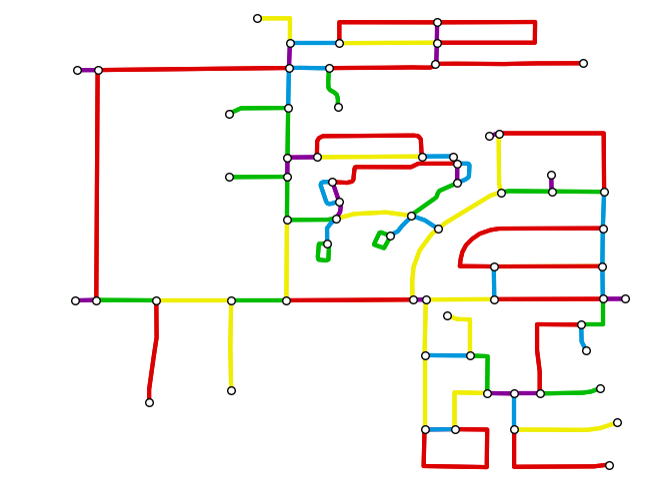
\includegraphics[width=0.4\textwidth]{figures/road-network.png} &
				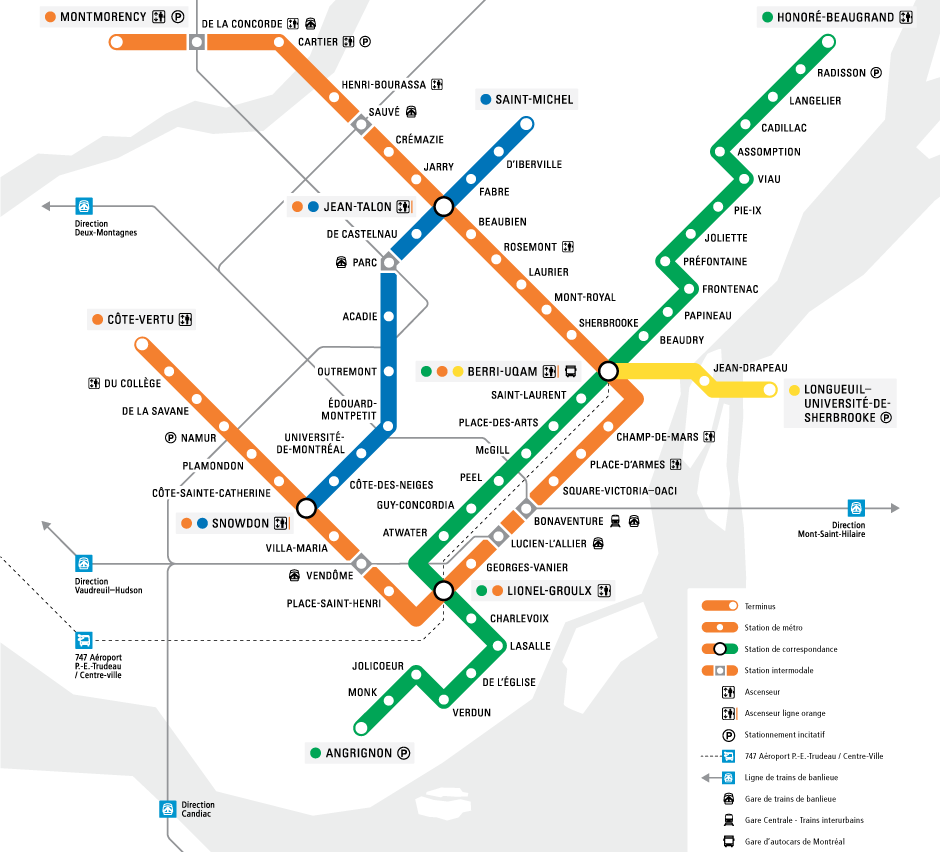
\includegraphics[width=0.4\textwidth]{figures/mtl-metro-cut.png} \\
			\end{tabular}
		\end{center}
		\caption{Example of a typical urban road-based network\footnotemark (left) and a subway route-based network\footnotemark (right).}
		\label{fig:networks}
	\end{figure*}
	
	\footnotetext[3]{Source: \cite{boeing2017osmnx}}
	\footnotetext{Source: \url{http://www.stm.info/fr/infos/reseaux/metro}}
	
	As these two contexts lead to different ways of structuring and querying the information, it is natural to expect at least two different representations, one for each context. For this reason, in this work we propose the use of compact data structures to design novel representations that are able to handle massive collections of data related to user transportation habits. We intend to cover both contexts, as well as offer a fair trade-off for different query needs, while at the same time ensuring that our proposals can be implemented in a real world scenario, for which we evaluate the performance of our representations with realistic query cases over real datasets\footnote{When needed, the real data was augmented or mixed with synthetic information}.
	
	Furthermore, as a proof of the practicability of our approach, we intend to develop a user interface that could enable the exploitation of this information by researchers, transportation companies, city administrations and any other kind of end users. This interface must, at the very least, allow visualizing the network elements on a map, also granting the ability to make queries over these elements in an intuitive and responsive way, while respecting the usual quality principles of any user-oriented software of this kind.
	
	In conclusion, we present an end-to-end platform around representations based on compact data structures to process, store, query and visualize mined public transportation usage data. To our knowledge, this is the first work to accomplish building such integrated platform, although other works exist that contemplate the use of compact data structures for trajectories or moving objects (see Section~\ref{sec:ti}).
	
	\section{Outline}
	This work is structured as follows...
	
\chapter{Related works}
	\section{Data mining}
	A couple of papers I have to copy from here and there to show that you can use smart cards, GPS or even cell network to track users. GPS is particularly useful in taxis. Cite that cool crowdsourcing approach with buses.
	
	\section{Trajectory indexing}
	\label{sec:ti}
	We can have that on networks or "free" spaces.
	
	\subsection{Free trajectory indexing}
	R-Tree perversion and Adrian's work.
	
	\subsection{Network constrained trajectory indexing}
	PARINET and Koide.
	
\chapter{Previous concepts}
	I am going to develop this more when I have more content on my proposals.
	
	\section{Summed Area Tables}
	The Summed Area Tables were first introduced in computer graphics \cite{crow1984summed} to speed up the mipmapping process.
	
	\section{Bitvectors}
	Rank and select.
	
	\section{Compressed Suffix Array (CSA)}
	Explaining ST and SA along the way.
	
	\section{Wavelet Tree and Wavelet Matrix}
	WM will be less confusing than in my previous paper...
	
	\section{Hu-Tucker coding}
	Which is like Huffman but preserving lexical order.
	
	\section{GIS interfaces}
	Because I have a web interface with leaflet after all.
	
	
\chapter{Contributions}
	As explained in Section~\ref{sec:pd}, there there are taxis and then there are buses. Their nature is different because of networks, so they must be treated differently. In the following sections we are going to propose representations for them both and then an interface for the buses case.
	
	\section{Representations for public transportation over streets}
	Old ass CTR \cite{brisaboa2018compact} with a WM or WT for times, and we tried different approaches to compress those times. It is not very useful for buses and metro because of the crazy redundancy.
	
	\subsection{Description}
	We have a CSA (with a twist) and then we align sampled times. We did introduce a Hu-Tucker WT tho...
	
	\subsection{Algorithms}
	We have X to Y and even Top K queries that are not that hard to describe.
	
	\subsection{Experiments}
	We may have not compared it to anything but we sure do have tons of results!
	
	\section{Representations for public transportation over networks}
	Here we speak about TTCTR and XCTR, where we have a network description and index journeys instead of explicit times.
	
	\subsection{Description}
	A network representation, then CSA for stops. In TTCTR we encode lines in these stops, while in XCTR we make the twist from before (I think) and then separate lines into a WM. Whatever the case, we then have an aligned WM of journeys. Oh and T-Matrices as a DW-like structure.
	
	\subsection{Algorithms}
	A bit complex for both TTCTR and XCTR. Maybe copy the complexity table from the paper that explains why TTCTR sucks for some queries and we needed to develop XCTR.
	
	\subsection{Experiments}
	Here we compare one to the other. Maybe include query times for postgresql, maybe later.
	
	\section{GIS interface for public transportation over networks}
	The tool we have developed that can interact with the previously described structures. We retell what we explained about GIS in previous concepts, and explain that this is different because it is built around our representations.
	
	\subsection{Analysis}
	From a functional perspective and then a technological one.
	
	\subsection{API}
	A nice and easy way to make queries and return data.
	
	\subsection{Interface}
	With a lot of screencaps that are going to take like 10 pages! Maybe even an evaluation section (which would require me to make it actually work well!).
	
\chapter{ Conclusions and future works}
	2-3 pages to speak about lessons learned and where is this all going.

% \nocite{*}
% \bibliographystyle{apalike}
\bibliographystyle{alpha}
\addcontentsline{toc}{chapter}{\bibname}
\bibliography{thesis}

\vfill \pagebreak \thispagestyle{empty} \mbox{}
\vfill \pagebreak \mbox{} \thispagestyle{empty}

\end{document}
%###
